\documentclass{scrartcl}
\usepackage[utf8]{inputenc}
\usepackage{hyperref}
\usepackage{url}
\usepackage{natbib}
\usepackage{graphicx}
\usepackage{cleveref} % this must be the last package to be loaded

\newcommand{\emailaddr}[1]{\href{mailto:#1}{\texttt{#1}}}

\title{\LARGE
    Distributed Audio Processing Pipeline with Observability
}
\subtitle{Final Report for the Distributed Systems Course AY 2025/2026}

\author{
    Matteo Cardellini \\ \emailaddr{matteo.cardellini@studio.unibo.it}
}

\date{\today}

\begin{document}

\maketitle

\begin{abstract} % max 2000 characters

This work presents a distributed, event-driven pipeline for asynchronous audio processing, designed as a practical case study for distributed systems principles and operational observability.

Users submit audio files through a FastAPI service. The API stores binary objects in MinIO, persists job metadata in PostgreSQL, and publishes processing requests to RabbitMQ. A decoupled worker consumes queued jobs, extracts core audio metadata (duration, sample rate, channels), and writes results back to the database. The same API exposes upload, job tracking, and result retrieval endpoints, enabling a complete end-to-end workflow.

The architecture separates ingestion and processing through asynchronous messaging, so API and worker instances can scale independently. Reliability is modeled through durable queue-based communication and explicit job-state transitions (PENDING, PROCESSING, DONE, FAILED), while observability is supported via Prometheus-compatible metrics for throughput, latency, queue backlog, and worker activity.

The stack is containerized with Docker and structured for Kubernetes-based deployment and scaling experiments. The project shows how message-driven coordination, persistent state management, and monitoring can be combined into a reproducible distributed audio-processing system.

\end{abstract}

\section*{Disclaimer (if needed)}

During the preparation of this work, the author used GitHub Copilot for language refinement and drafting support.
All technical choices, validation activities, and final content were reviewed and approved by the author, who takes full responsibility for the report.

% \section*{Quick \LaTeX{} suggestions}

% If you need to cite a reference, you can use the \texttt{cite} command, 
% like providing the BibTex key of some entry in the \texttt{references.bib} file, 
% e.g.: \cite{adams1995hitchhiker}.

% You can find pre-coocked BibTex entries for most Computer Science papers on \href{https://dblp.uni-trier.de/}{DBLP}.

% If you need to include an image,
% let \LaTeX{} decide where to put it by using the \texttt{figure} environment,
% with a \texttt{includegraphics} command inside it.
% %
% If your need to reference a figure,
% use the \texttt{label} command to assign a label to the figure,
% and then use the \texttt{cref} command to reference it.
% %
% Put figures in the \texttt{figures} folder.
% %
% A complete example is shown in \cref{fig:universe}.

% \begin{figure}
%     \centering
%     
\includegraphics[width=0.5\textwidth]{figures/universe.jpg}
%     \caption{This is an example image}
%     \label{fig:universe}
% \end{figure}

% Do \textbf{not} put any placement constraint on figures,
% such as \texttt{[h]} or \texttt{[h!]}.
% %
% Same considerations apply for other floating elements 
% (e.g. tables, algorithms, listings, etc.).

% Do \textbf{not} use the \texttt{\textbackslash\textbackslash} or \texttt{\textbackslash newline} commands to break lines.

% Just leave an empty line between two paragraphs to start a new one.
% %
% The new line will be automatically indented.
% %
% This is intended: it is the \LaTeX{} way to separate capoverses.

\section{Concept}\label{concept}

\subsection*{Type of Product}

% \begin{itemize}
%   \item The type of product developed with that project, for example (non-exhaustive):
%   %
%   \begin{itemize}
%     \item Application (with GUI, be it mobile, web, or desktop)
%     \item Command-line application (CLI could be used by humans or scripts)
%     \item Library
%     \item Web-service(s)
%   \end{itemize}

The developed product is a \textbf{distributed, service-oriented application} for asynchronous audio processing.
From an architectural perspective, it is composed of \textbf{three cooperating software components}:

\begin{itemize}
  \item a \textbf{web API} (FastAPI) that exposes upload, job-status, and result-retrieval endpoints;
  \item a \textbf{background worker service} that consumes queued jobs and executes audio processing tasks;
  \item a \textbf{lightweight browser-based frontend} used as an interactive client for manual usage and demo scenarios.
\end{itemize}

Therefore, the project is primarily a distributed web-service system, complemented by a simple web application for user interaction, rather than a standalone library or CLI-only tool.

\subsection*{Use Case Description}

%   \item Use case description:
%   %
%   \begin{itemize}
%     \item \emph{what} is the software doing?
%     \item \emph{where} are the users?
%     \item \emph{when} and \emph{how frequently} do they interact with the system?
%     \item \emph{how} do they \emph{interact} with the system? which \emph{devices} are they using?
%     \item does the system need to \emph{store} user's \textbf{data}? \emph{which}? \emph{where}?
%     \item most likely, there will be \emph{multiple} \textbf{roles}
%   \end{itemize}

The system supports \textbf{asynchronous audio-processing requests} submitted by users through an HTTP API.
In a typical scenario, a user uploads an audio file, receives a \textbf{job identifier}, and later queries the job state and extracted results.
This interaction model avoids long synchronous waits and is suitable for workloads where processing time is variable.

Users access the platform remotely through a web browser or an API client, typically from personal computers and, when needed, from mobile devices with HTTP-capable tools.
Interaction frequency is naturally bursty: short upload sessions can generate multiple jobs in sequence, followed by periodic status checks until processing completes.

The platform stores both \textbf{binary} and \textbf{structured} data.
Audio files are persisted in object storage (MinIO), while job metadata and processing outcomes are persisted in PostgreSQL.
Stored information includes job identifiers, file references, processing states, timestamps, and extracted audio metadata such as duration, sample rate, and number of channels.

At the architectural level, the system involves distinct roles: client users submitting requests, the API service coordinating ingestion and orchestration, and worker services executing background processing.
This role separation is a core part of the distributed use case and enables clearer responsibility boundaries across components.

\subsection*{Why Distribution Is Needed}

%   \item Why is distribution needed?
%   %
%   \begin{itemize}
%     \item geographically distributed environments?
%     \item computation speedup?
%     \item resource sharing?
%     \item fault tolerance?
%     \item other reasons?
%   \end{itemize}
%   %
%   In any case, please elaborate.
% \end{itemize}

Distribution is a \textbf{structural requirement} of this project, not only an implementation preference.
Audio processing tasks can take variable and non-trivial execution time, so coupling upload handling and processing in a single synchronous component would reduce responsiveness and limit throughput.
By separating ingestion (API) from execution (workers) through a message broker, the system can accept requests quickly and process them asynchronously.

This design enables \textbf{independent horizontal scaling} of components: API instances can scale to absorb request bursts, while worker replicas can scale according to queue backlog and processing demand.
It also promotes resource sharing, since multiple workers consume from the same queue and operate on a common persistent state stored in PostgreSQL and MinIO.

Distribution also improves \textbf{fault isolation} and operational resilience.
If a worker instance fails during processing, new requests can still be accepted by the API, and queued jobs remain available for other workers.
Combined with explicit job-state transitions and persistent storage, this model provides a robust foundation for reliability, observability, and incremental system evolution.

\section{Requirements Elicitation and Analysis}\label{requirements}

% \begin{itemize}
%   \item The requirements must explain \textbf{what} (not how) the software
%   being produced should do.
%   %
%   \begin{itemize}
%     \item you should not focus on the particular problems, but exclusively on
%     what you want the application to do.
%   \end{itemize}

%   \item Requirements must be clearly identified, and possibly numbered

%   \item Requirements are divided into:
%   %
%   \begin{itemize}
%     \item \textbf{Functional}: some functionality the software should provide to the user

%     \item \textbf{Non-functional}: requirements that do not directly concern behavioural aspects, such as consistency, availability, etc.

%     \item \textbf{Implementation}: constrain the entire phase of system realization,
%     for instance by requiring the use of a specific programming language and/or a specific software tool
%     %
%     \begin{itemize}
%       \item these constraints should be adequately justified by political / economic / administrative reasons\ldots{}
%       \item \ldots{} otherwise, implementation choices should emerge \emph{as  a consequence of} design
%     \end{itemize}
%   \end{itemize}

%   \item If there are domain-specific terms, these should be explained in a glossary

%   \item Each requirement must have its own \textbf{acceptance criterion}
%   %
%   \begin{itemize}
%     \item these will be important for the validation phase
%   \end{itemize}
% \end{itemize}

This section defines \textbf{what} the system must provide from a functional and quality perspective.
Requirements are identified with unique IDs and paired with explicit acceptance criteria used later in validation.

\subsection*{Glossary}

\begin{itemize}
  \item \textbf{Job}: one asynchronous processing request created after an audio upload.
  \item \textbf{Job state}: lifecycle value associated with a job (PENDING, PROCESSING, DONE, FAILED).
  \item \textbf{Queue backlog}: number of jobs waiting to be processed by workers.
  \item \textbf{Processing result}: extracted audio metadata returned by the worker and persisted by the platform.
\end{itemize}

\subsection*{Functional Requirements}

\begin{itemize}
  \item \textbf{FR1: Audio upload}. The system shall allow a user to submit an audio file and create a processing job.
  \textbf{Acceptance criterion:} after a valid upload request, the API returns success with a new job identifier and an initial job state.

  \item \textbf{FR2: Asynchronous execution}. The system shall execute audio processing asynchronously with respect to request submission.
  \textbf{Acceptance criterion:} upload requests complete without waiting for final processing, while the corresponding job continues in background.

  \item \textbf{FR3: Job status retrieval}. The system shall expose an endpoint to retrieve the current state of a job by identifier.
  \textbf{Acceptance criterion:} querying an existing job returns one valid state among PENDING, PROCESSING, DONE, FAILED.

  \item \textbf{FR4: Result retrieval}. The system shall expose an endpoint to retrieve processing results when available.
  \textbf{Acceptance criterion:} for jobs in DONE state, the API returns persisted extracted metadata; for unfinished jobs, it returns a consistent status response.

  \item \textbf{FR5: Persistent storage}. The system shall persist uploaded audio objects and job metadata.
  \textbf{Acceptance criterion:} after restart of application containers, previously created jobs and stored files remain available.

  \item \textbf{FR6: Failure visibility}. The system shall make processing failures observable through job state and error information.
  \textbf{Acceptance criterion:} if processing fails, the job is marked FAILED and failure details are retrievable through API/database inspection.
\end{itemize}

\subsection*{Non-Functional Requirements}

\begin{itemize}
  \item \textbf{NFR1: Scalability}. The system should support horizontal scaling of API and worker components.
  \textbf{Acceptance criterion:} increasing worker replicas increases processing throughput under comparable load.

  \item \textbf{NFR2: Responsiveness}. Upload operations should remain fast even when processing is slow.
  \textbf{Acceptance criterion:} upload endpoint remains responsive because processing is decoupled and queued.

  \item \textbf{NFR3: Reliability}. Jobs should not be lost during normal component restarts or transient worker issues.
  \textbf{Acceptance criterion:} queued or persisted jobs are recoverable and continue through lifecycle after restart.

  \item \textbf{NFR4: Observability}. The platform should expose measurable operational signals.
  \textbf{Acceptance criterion:} Prometheus-compatible metrics for requests, processing activity, and failures are exposed by services.

  \item \textbf{NFR5: Maintainability}. The architecture should keep service responsibilities clearly separated.
  \textbf{Acceptance criterion:} API and worker can be developed, deployed, and scaled independently without changing external contract.
\end{itemize}

\subsection*{Implementation Constraints}

\begin{itemize}
  \item \textbf{IR1: Service implementation language}. Core services shall be implemented in Python.
  \textbf{Acceptance criterion:} API and worker codebases are Python projects with reproducible dependency management.

  \item \textbf{IR2: Messaging middleware}. Asynchronous coordination shall use RabbitMQ.
  \textbf{Acceptance criterion:} job dispatch and consumption happen through RabbitMQ queues/exchanges.

  \item \textbf{IR3: Data technologies}. Job metadata shall be persisted in PostgreSQL and audio objects in MinIO.
  \textbf{Acceptance criterion:} no alternative primary store is required for the main pipeline flow.

  \item \textbf{IR4: Containerized deployment}. Services shall be runnable via container orchestration for reproducibility.
  \textbf{Acceptance criterion:} the full stack can be started with Docker Compose and deployed to Kubernetes manifests/charts provided in the repository.
\end{itemize}



\subsection{Relevant Distributed System Features}
\label{ds-features}

% Motivate which distributed system features are relevant for your project, and which are not.
% %
% \begin{itemize}
%   \item transparency
%   \begin{itemize}
%     \item does your system need to hide distribution details from users or developers?
%     \item is it important that failures, location, or replication are invisible?
%   \end{itemize}

%   \item fault tolerance, dependability -- availability, reliability, integrity, maintainability, safety
%   \begin{itemize}
%     \item what happens if a component fails? is uninterrupted service required?
%     \item is data loss or corruption unacceptable?
%     \item how quickly must the system recover from faults?
%   \end{itemize}

%   \item scalability
%   \begin{itemize}
%     \item will the system need to handle increasing numbers of users, requests, or data?
%     \item is it expected to grow over time?
%   \end{itemize}

%   \item security, trust
%   \begin{itemize}
%     \item is sensitive data being processed or stored?
%     \item are there multiple user roles with different permissions?
%     \item is authentication or authorization required?
%   \end{itemize}

%   \item resource sharing
%   \begin{itemize}
%     \item do multiple users or components need access to shared resources?
%     \item is coordination or synchronization needed?
%   \end{itemize}

%   \item openness, interoperability, heterogeneity of components
%   \begin{itemize}
%     \item Will your system interact with external systems or use components built with different technologies?
%     \item Is standardization or compatibility important?
%   \end{itemize}

%   \item evolvability, maintainability
%   \begin{itemize}
%     \item Will the system need to be updated or extended after deployment?
%     \item Is long-term maintenance a concern?
%   \end{itemize}

%   \item performance, concurrency, computation / communication efficiency, bandwidth
%   \begin{itemize}
%     \item Are there strict requirements on response time or throughput?
%     \item Will many operations happen in parallel?
%     \item Is network usage a concern?
%   \end{itemize}

%   \item economy, costs
%   \begin{itemize}
%     \item Are there budget constraints for development, deployment, or operation?
%     \item Is minimizing resource usage important?
%   \end{itemize}
% \end{itemize}

For this project, distributed-system features have different priorities.

\begin{itemize}
  \item \textbf{Scalability (high relevance).} The pipeline must absorb burst uploads and variable processing demand.
  Independent scaling of API and workers is therefore essential.

  \item \textbf{Fault tolerance and dependability (high relevance).} Worker or network issues must not cause immediate job loss.
  Durable messaging, persistent state, and explicit job transitions are central to reliability.

  \item \textbf{Resource sharing (high relevance).} Multiple workers share queue workload and common storage backends.
  Coordination around shared queue and shared state is intrinsic to the architecture.

  \item \textbf{Performance and concurrency (high relevance).} Many jobs may execute concurrently, and throughput under load is a key quality objective.

  \item \textbf{Evolvability and maintainability (high relevance).} Service separation enables incremental changes (API, worker, observability) with limited cross-impact.

  \item \textbf{Security and trust (medium relevance).} The system includes authentication and controlled API access, but it is not designed for highly sensitive regulated workloads.

  \item \textbf{Transparency (medium relevance).} Users are abstracted from internal distribution details, but operational distribution remains explicit for developers and operators.

  \item \textbf{Openness and interoperability (medium relevance).} The system relies on widely adopted protocols and components (HTTP, AMQP, SQL), which simplifies integration and portability.

  \item \textbf{Economy and costs (medium relevance).} Containerization and local orchestration reduce setup and experimentation costs while preserving realistic deployment patterns.
\end{itemize}

\section{Design}\label{design}

% This chapter explains the strategies used to meet the requirements identified in the analysis. 

% Ideally, the design should be the same, regardless of the technological choices made during the implementation phase.

% \begin{quote}
% You can re-arrange the sections as you prefer, but all the sections must be present in the end
% \end{quote}

% \noindent
% \textbf{Important:} try to motivate your design choices in relation to the requirements and features identified 
% in \cref{requirements} and \cref{ds-features}.

This section describes how the system design addresses the requirements in \cref{requirements}, with a focus on
scalability, fault isolation, resource sharing, and observability.
The architecture is message-driven: ingestion, background processing, and persistence are separated into dedicated
components so each part can evolve and scale independently.
This separation keeps API requests responsive under load, while worker capacity can increase as queue backlog grows.
Components coordinate asynchronously through explicit job lifecycle states persisted in shared storage.

The next subsections present the design in order: architectural style, infrastructure, modelling, interaction,
behaviour, data consistency, fault tolerance, availability, and security.

\subsection{Architecture}\label{architecture}

% \begin{itemize}
%   \item Which architectural style?
%   %
%   \begin{itemize}
%     \item why?
%   \end{itemize}
% \end{itemize}

\begin{figure}
  \centering
  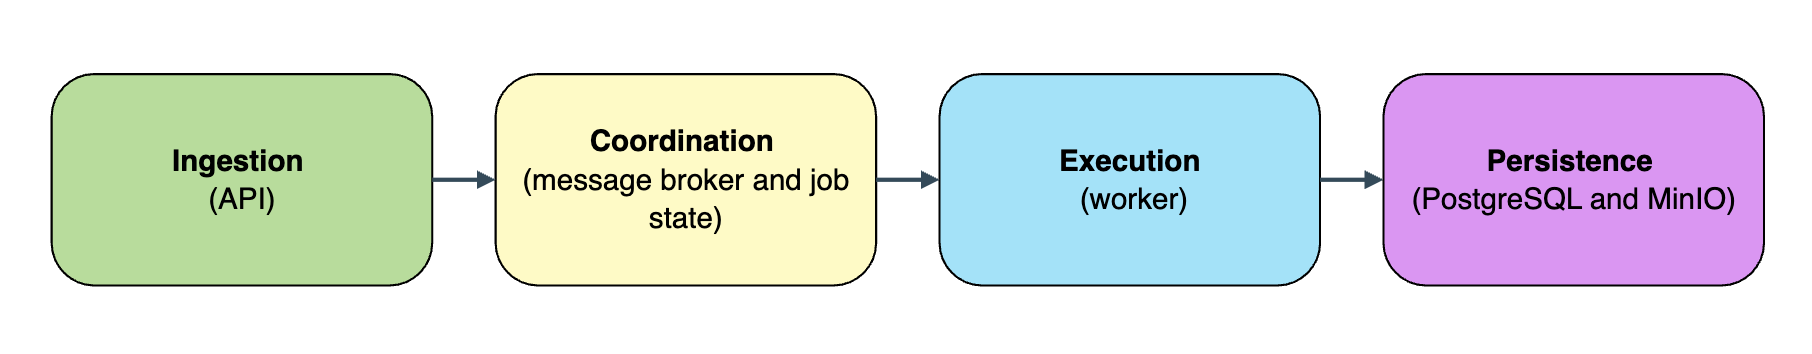
\includegraphics[width=1.0\textwidth]{figures/architecture-pipeline.png}
  \caption{Four-block pipeline: ingestion, coordination, execution, and persistence.}
  \label{fig:pipeline-overview}
\end{figure}

The system follows an \textbf{event-driven, service-oriented architecture}.
It combines two interaction styles:

\begin{itemize}
  \item \textbf{synchronous request-response} for user-facing API operations (upload, status, result retrieval);
  \item \textbf{asynchronous message-driven processing} for background job execution through RabbitMQ.
\end{itemize}

This architectural style was chosen to satisfy the most important requirements.
First, it keeps the API responsive because request handling is separated from long-running processing tasks.
Second, it enables independent scaling of API and worker components, which directly supports throughput growth under variable load.
Third, it improves fault isolation: temporary worker issues do not block request intake, and queued jobs remain processable by other workers.

In practical terms, the architecture can be seen as a small pipeline with clear stages:
\textbf{ingestion} (API), \textbf{coordination} (message broker and job state), \textbf{execution} (worker), and \textbf{persistence} (PostgreSQL and MinIO).
This separation also improves maintainability, since each stage can evolve with limited impact on the others.
A visual summary of this \textbf{four-block pipeline} is shown in \cref{fig:pipeline-overview}.

\subsection{Infrastructure}\label{infrastructure}

% \begin{itemize}
%   \item are there \emph{infrastructural components} that need to be introduced? \emph{how many}?
%   %
%   \begin{itemize}
%     \item e.g.~\emph{clients}, \emph{servers}, \emph{load balancers},
%     \emph{caches}, \emph{databases}, \emph{message brokers},
%     \emph{queues}, \emph{workers}, \emph{proxies}, \emph{firewalls},
%     \emph{CDNs}, \emph{etc.}
%   \end{itemize}

%   \item how do components \emph{distribute} over the network? \emph{where}?
%   %
%   \begin{itemize}
%     \item e.g.~do servers / brokers / databases / etc. sit on the same
%     machine? on the same network? on the same datacenter? on the same
%     continent?
%   \end{itemize}

%   \item how do components \emph{find} each other?
%   %
%   \begin{itemize}
%     \item how to \emph{name} components?
%     \item e.g.~DNS, \emph{service discovery}, \emph{load balancing},
%     \emph{etc.}
%   \end{itemize}
% \end{itemize}

% \begin{quote}
% Component diagrams are welcome here
% \end{quote}

\begin{figure}
  \centering
  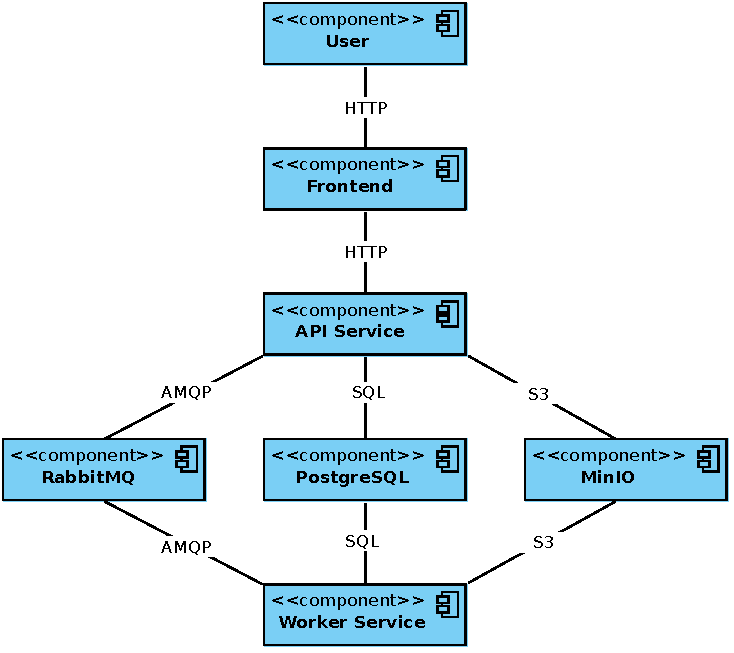
\includegraphics[width=0.7\textwidth]{figures/component-diagram.pdf}
  \caption{Runtime components and their communication protocols.}
  \label{fig:components}
\end{figure}

The infrastructure is built around six runtime components.
\Cref{fig:components} provides a simplified overview of their roles and primary communication protocols (HTTP, AMQP, SQL, S3).

\begin{itemize}
  \item \textbf{Frontend client}: a lightweight web interface for manual interaction;
  \item \textbf{API service}: handles HTTP requests, upload orchestration, and status/result queries;
  \item \textbf{Worker service}: consumes queued jobs and executes audio processing;
  \item \textbf{RabbitMQ}: message broker used for asynchronous coordination between API and workers;
  \item \textbf{PostgreSQL}: persistent relational store for job metadata and processing outcomes;
  \item \textbf{MinIO}: object storage for uploaded audio files.
\end{itemize}

Kubernetes is the default deployment model: each component runs as one or more pods, while Services provide stable endpoints for internal and external traffic.
This setup enables horizontal scaling of stateless parts, especially workers, without changing application logic.
Service discovery is DNS-based through Kubernetes Service names, which removes hard-coded addresses and improves portability.
Traffic distribution is handled by platform primitives: API HTTP requests are balanced at Service level, and processing load is distributed as workers compete for RabbitMQ messages.
An external load balancer remains optional, depending on the target cluster environment.

\subsection{Modelling}\label{modelling}

% \begin{itemize}
%   \item which \textbf{domain entities} are there?
%   %
%   \begin{itemize}
%     \item e.g.~\emph{users}, \emph{products}, \emph{orders}, \emph{etc.}
%   \end{itemize}
%   
%   \item how do \emph{domain entities} \textbf{map to} \emph{infrastructural components}?
%   %
%   \begin{itemize}
%     \item e.g.~state of a video game on central server, while inputs/representations on clients
%     \item e.g.~where to store messages in an IM app? for how long?
%   \end{itemize}

%   \item which \textbf{domain events} are there?
%   %
%   \begin{itemize}
%     \item e.g.~\emph{user registered}, \emph{product added to cart}, \emph{order placed}, \emph{etc.}
%   \end{itemize}
%   
%   \item which sorts of \textbf{messages} are exchanged?
%   %
%   \begin{itemize}
%     \item e.g.~\emph{commands}, \emph{events}, \emph{queries}, \emph{etc.}
%   \end{itemize}

%   \item what information does the \textbf{state} of the system comprehend
%   %
%   \begin{itemize}
%     \item e.g.~\emph{users' data}, \emph{products' data}, \emph{orders' data}, \emph{etc.}
%   \end{itemize}
% \end{itemize}

% \begin{quote}
% Class diagram are welcome here
% \end{quote}

\begin{figure} % BLUE = domain entities, GREEN = service / business logic, PURPLE = instructural components
  \centering
  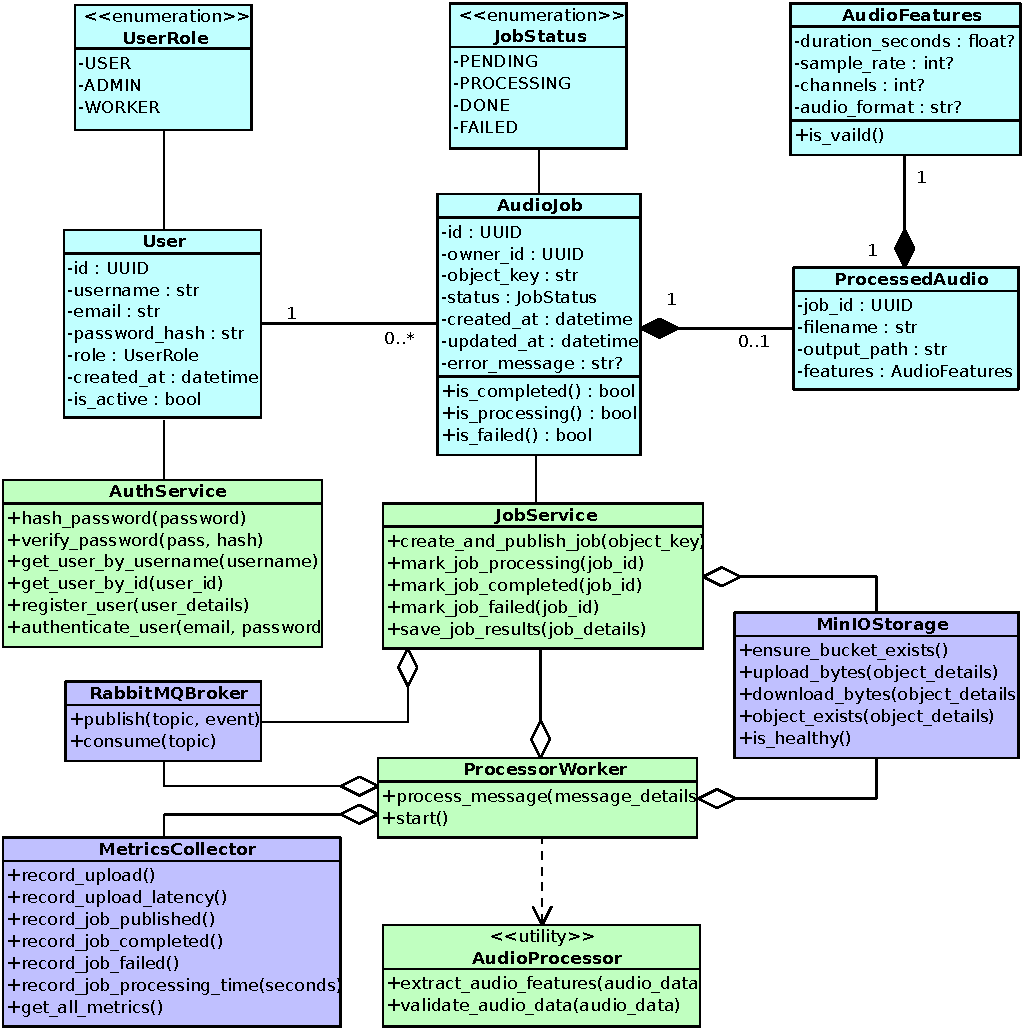
\includegraphics[width=1.0\textwidth]{figures/Class Diagram.pdf}
  \caption{Class diagram showing the main domain entities, their relationships, and how they map to infrastructural components.}
  \label{fig:class-diagram}
\end{figure}

\Cref{fig:class-diagram} captures the core domain model of the asynchronous pipeline.
The primary \textbf{domain entities} are \texttt{User}, \texttt{AudioJob}, and \texttt{ProcessedAudio}, with \texttt{AudioFeatures} as a value object associated with processing results.
In this model, each uploaded file creates exactly one \texttt{AudioJob}, identified by a unique ID, owned by a user, and tracked through the lifecycle states
\texttt{PENDING}, \texttt{PROCESSING}, \texttt{DONE}, and \texttt{FAILED}.
When processing completes successfully, \texttt{ProcessedAudio} stores extracted metadata such as duration, sample rate, and channel count.

\textbf{Entity-to-infrastructure mapping} follows component responsibilities.
Identity and job metadata are persisted in PostgreSQL, binary audio content is persisted in MinIO, and execution coordination is delegated to RabbitMQ.
At runtime, API-side services create jobs, validate access, and expose query operations, while worker-side services consume queued jobs,
execute processing logic, and apply lifecycle transitions to persistent state.

The \textbf{domain events} considered by the model are: \emph{job created}, \emph{job queued}, \emph{processing started}, \emph{processing completed}, and \emph{processing failed}.
These are reflected in three \textbf{message categories} exchanged among components:
\emph{commands} (e.g., enqueue processing), \emph{events} (state transitions), and \emph{queries} (status and result retrieval).

The \textbf{overall system state} includes user identity and role data, job ownership and lifecycle metadata,
object-storage references, extracted audio features, timestamps, and error diagnostics.
This state is intentionally externalized in durable stores so that execution remains recoverable after restarts
and observable across API and worker components.


\subsection{Interaction}\label{interaction}

% \begin{itemize}
%   \item how do components \emph{communicate}? \emph{when}? \emph{what}?
%   \item \emph{which} \textbf{interaction patterns} do they enact?
% \end{itemize}

% \begin{quote}
% Sequence diagrams are welcome here
% \end{quote}

Component interaction is structured around four recurrent runtime flows that cover the complete user-facing lifecycle:
authentication, upload and job creation, background processing, and status/result retrieval.
Within these flows, synchronous HTTP is used for client-facing request-response operations,
whereas asynchronous AMQP messaging decouples ingestion from execution between API and workers.
This hybrid interaction model provides immediate feedback to clients while allowing processing to complete in the background.

\subsubsection*{Flow 1: Authentication (register and login)}

\begin{figure}
  \centering
  
\includegraphics[width=1.0\textwidth]{\detokenize{figures/sequence-flow/Authentication Flow (Register & Login).pdf}}
  \caption{Sequence for user registration and login, leading to JWT issuance and authenticated API usage.}
  \label{fig:seq-auth}
\end{figure}

As shown in \cref{fig:seq-auth}, a new user first registers through the API.
The service validates the payload, persists the user in PostgreSQL, and returns a successful registration response.
For subsequent access, the login request triggers credential verification followed by JWT issuance.
The client then includes the token in the \texttt{Authorization} header when invoking protected endpoints.

\subsubsection*{Flow 2: Upload and job creation}

\begin{figure}
  \centering
  
\includegraphics[width=1.0\textwidth]{\detokenize{figures/sequence-flow/Upload & Job Creation Flow.pdf}}
  \caption{Sequence for file upload, persistent job creation, and asynchronous dispatch to the processing queue.}
  \label{fig:seq-upload}
\end{figure}

In \cref{fig:seq-upload}, an authenticated client uploads an audio file to the API.
The API stores the binary object in MinIO, creates the corresponding \texttt{AudioJob} in PostgreSQL with initial state \texttt{PENDING},
and publishes a processing command to RabbitMQ.
The client receives the job identifier immediately; therefore, request latency is independent of processing time.
This is the primary ingestion path and the main integration point between synchronous and asynchronous communication.

\subsubsection*{Flow 3: Worker processing}

\begin{figure}
  \centering
  
\includegraphics[width=1.0\textwidth]{\detokenize{figures/sequence-flow/Worker Processing Flow.pdf}}
  \caption{Sequence for queue consumption, processing execution, and final state transition update.}
  \label{fig:seq-worker}
\end{figure}

\Cref{fig:seq-worker} details the execution path after a message becomes available in RabbitMQ.
The worker consumes the job message, updates the job state to \texttt{PROCESSING}, fetches the source object from MinIO,
extracts audio metadata, and persists outputs in PostgreSQL.
On success, the state transitions to \texttt{DONE}; on failure, it transitions to \texttt{FAILED} with diagnostic details.
Broker acknowledgement is sent only after the processing attempt is finalized, supporting robust at-least-once consumption semantics.

\subsubsection*{Flow 4: Job status and result retrieval}

\begin{figure}
  \centering
  
\includegraphics[width=1.0\textwidth]{\detokenize{figures/sequence-flow/Job Status & Results Retrieval Flow.pdf}}
  \caption{Sequence for polling job status and retrieving processing results once completion is reached.}
  \label{fig:seq-status}
\end{figure}

Finally, \cref{fig:seq-status} describes the read path used after submission.
The client periodically queries job status through the API, which retrieves the current lifecycle value from PostgreSQL.
While processing is ongoing, the API returns consistent intermediate responses; once the state is \texttt{DONE},
the result endpoint returns persisted metadata (duration, sample rate, channels).

Taken together, these four flows implement a coherent interaction pattern:
state-changing ingestion operations remain short and synchronous,
compute-intensive work is decoupled and asynchronous,
and completion is exposed through explicit state queries.

\subsection{Behaviour}\label{behaviour}

% \begin{itemize}
%   \item how does \emph{each} component \textbf{behave} individually (e.g.~in \emph{response} to \emph{events} or messages)?
%   \begin{itemize}
%     \item some components may be \emph{stateful}, others \emph{stateless}
%   \end{itemize}

%   \item which components are in charge of updating the \textbf{state} of the system? \emph{when}? \emph{how}?
% \end{itemize}

% \begin{quote}
% State diagrams are welcome here
% \end{quote}

Behaviour in this system is centered on two complementary state machines.
The first one describes the \textbf{business lifecycle} of an \texttt{AudioJob}, while the second one describes the \textbf{runtime behavior} of the worker while it consumes and processes queue messages.
Together, they clarify which component updates state, which state is persistent, and which state is only internal to execution.

\begin{figure}
  \centering
  
\includegraphics[width=1.0\textwidth]{\detokenize{figures/state-diagrams/State Diagram - AudioJob lifecycle.pdf}}
  \caption{State diagram for the \texttt{AudioJob} lifecycle, from creation to completion or failure.}
  \label{fig:state-job-lifecycle}
\end{figure}

\Cref{fig:state-job-lifecycle} shows the persistent job lifecycle stored in PostgreSQL.
When the API receives a valid upload, it creates the job in \texttt{PENDING} state.
The worker then advances the job to \texttt{PROCESSING} when it starts consuming the corresponding message.
If the processing succeeds, the job becomes \texttt{DONE} and the extracted metadata are persisted.
If the processing fails, the job is either retried or, after the retry budget is exhausted, marked \texttt{FAILED}.
These terminal states are terminal only for the job record; they do not stop the service itself.

\begin{figure}
  \centering
  
\includegraphics[width=1.0\textwidth]{\detokenize{figures/state-diagrams/State Diagram - Worker Logic.pdf}}
  \caption{State diagram for the worker execution loop, including bounded retry handling.}
  \label{fig:state-worker-logic}
\end{figure}

\Cref{fig:state-worker-logic} captures the internal control flow of the worker service.
The worker is intentionally long-running and therefore does not have a final lifecycle state in the usual sense: after handling one message, it returns to its idle listening state and waits for the next one.
This diagram models a single message-processing cycle, starting from message reception, moving through parsing and processing, and then branching either to successful completion or to retry scheduling.
On transient failures, the worker republishes the message with an incremented attempt counter and resets the job to \texttt{PENDING}; once the retry limit is reached, the worker records the final failure and stops retrying that job.

\subsection{Data and Consistency Issues}\label{data-and-consistency-issues}

% \begin{itemize}
%   \item Is there any data that needs to be stored?
%   %
%   \begin{itemize}
%     \item \emph{what} data? \emph{where}? \emph{why}?
%   \end{itemize}
  
%   \item how should \emph{persistent data} be \textbf{stored}?
%   %
%   \begin{itemize}
%     \item e.g.~relations, documents, key-value, graph, etc.
%     \item why?
%   \end{itemize}
  
%   \item Which components perform queries on the database?
%   %
%   \begin{itemize}
%     \item \emph{when}? \emph{which} queries? \emph{why}?
%     \item concurrent read? concurrent write? why?
%   \end{itemize}
  
%   \item Is there any data that needs to be shared between components?
%   %
%   \begin{itemize}
%     \item \emph{why}? \emph{what} data?
%   \end{itemize}
% \end{itemize}

The system stores both \textbf{persistent business data} and \textbf{ephemeral coordination data}.
Persistent business data includes user accounts, authentication-related information, job metadata, job ownership, job state transitions, error messages, and extracted audio results.
Binary audio files are not stored in the relational database: they are persisted separately in MinIO as objects, while PostgreSQL keeps only the references needed to reconstruct the processing flow.
This separation keeps the relational model compact and makes large file handling independent from metadata queries.

Persistent data is modeled as a relational schema because the main entities have clear identifiers, strong relationships, and structured lifecycle transitions.
PostgreSQL is therefore the source of truth for users, jobs, and processing outcomes (as illustrated in Figure~\ref{fig:er-diagram}), while MinIO is the source of truth for uploaded audio content.
The message broker is intentionally not used as the system of record: RabbitMQ carries work commands, but the durable state is always reconstructed from the database and object storage.

Several components perform queries on the database, but they do so with different responsibilities.
The API service writes user and job data during registration, authentication, and upload handling, then reads jobs and results when serving status or result requests.
The worker service updates job state during execution and writes processing results after a successful extraction attempt.
Because the worker and API may access the same records concurrently, the design favors small, explicit updates rather than long transactions spanning multiple components.

Concurrent access is mostly read-heavy, with writes concentrated on job creation, status transitions, and result persistence.
The main contention point is the \texttt{jobs} table, since the API initializes jobs and the worker advances their state.
This is acceptable because each job is updated by a small number of transitions and the transitions are monotonic in normal execution.
The \texttt{processing\_results} table is updated with an upsert pattern, which keeps retries idempotent and avoids duplicate result rows when a message is reprocessed.

Some data must be shared between components, but only through durable storage and message payloads.
The shared identifiers are the job ID, owner ID, storage object key, current state, timestamps, and extracted features.
AMQP messages carry the job ID, object key, and retry attempt counter so the worker can continue execution without embedding business state in the queue itself.

\begin{figure}
\centering
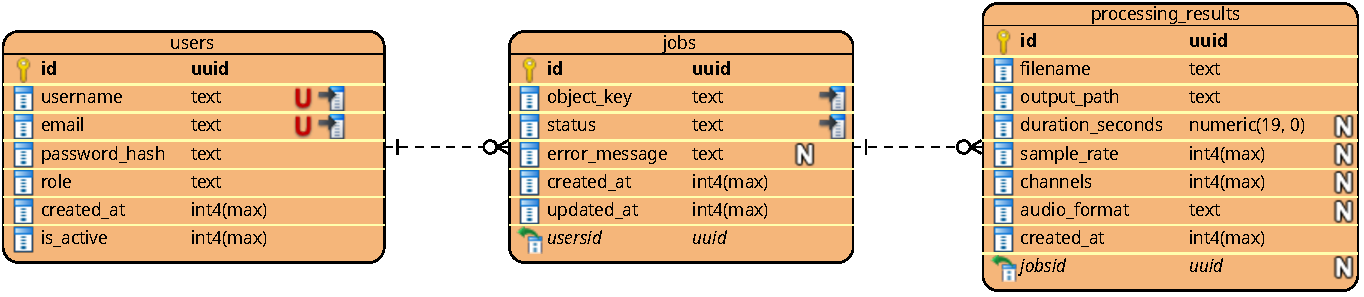
\includegraphics[width=1.0\textwidth]{figures/ER Diagram.pdf}
\caption{PostgreSQL schema entities and relationships.}
\label{fig:er-diagram}
\end{figure}


\subsection{Fault-Tolerance}\label{fault-tolerance}

\begin{itemize}
  \item Is there any form of data \textbf{replication} / federation / sharing?
  %
  \begin{itemize}
    \item \emph{why}? \emph{how} does it work?
  \end{itemize}
  
  \item Is there any \textbf{heart-beating}, \textbf{timeout}, \textbf{retry mechanism}?
  %
  \begin{itemize}
    \item \emph{why}? \emph{among} which components? \emph{how} does it work?
  \end{itemize}
  
  \item Is there any form of \textbf{error handling}?
  %
  \begin{itemize}
    \item \emph{what} happens when a component fails? \emph{why}? \emph{how}?
  \end{itemize}
\end{itemize}

\subsection{Availability}\label{availability}

\begin{itemize}
  \item Is there any \textbf{caching} mechanism?
  %
  \begin{itemize}
    \item \emph{where}? \emph{why}?
  \end{itemize}
  
  \item Is there any form of \textbf{load balancing}?
  %
  \begin{itemize}
    \item \emph{where}? \emph{why}?
  \end{itemize}

  \item In case of \textbf{network partitioning}, how does the system behave?
  %
  \begin{itemize}
    \item \emph{why}? \emph{how}?
  \end{itemize}
\end{itemize}

\subsection{Security}\label{security}

The system implements \textbf{stateless, token-based authentication} and \textbf{role-based access control} to protect API endpoints and ensure that users can only access their own resources.

\subsubsection*{Authentication}

Authentication is realized through \textbf{JWT (JSON Web Tokens)} issued on successful login.
When a user submits valid credentials (username and password), the API verifies them against the stored password hash and issues a JWT token.
The token is signed using the HS256 algorithm and contains the user ID as the subject and an expiration time.
The client includes the token in the \texttt{Authorization} header as a bearer token for all subsequent requests.
Each protected endpoint applies a dependency that extracts and validates the token, extracting the user ID and loading the corresponding user record from the database.
If the token is missing, malformed, or expired, the request is rejected with a 401 Unauthorized response.
This approach keeps authentication stateless and allows API instances to verify tokens without session storage or coordination.

\subsubsection*{Authorization}

The system uses \textbf{role-based access control (RBAC)} with three defined roles: \texttt{USER}, \texttt{ADMIN}, and \texttt{WORKER}.
Standard users are granted the \texttt{USER} role on registration and can submit audio files, retrieve their own job status, and view their processing results.
Job ownership is enforced at the application layer: queries filter results by the authenticated user's ID, so users can only see and interact with jobs they created.
Administrative operations (user management, system configuration) are restricted to instances with the \texttt{ADMIN} role.
The \texttt{WORKER} role is reserved for internal service-to-service communication in scenarios requiring explicit worker identification; it is not assigned to regular users.
Authorization checks are implemented as FastAPI dependency injection, which transparently enforces access rules at the route level.

\subsubsection*{Cryptographic Schemas}

The system employs two complementary cryptographic mechanisms:
\begin{itemize}
  \item \textbf{Password hashing}: User passwords are hashed using bcrypt before storage in PostgreSQL. This ensures that even if the database is compromised, passwords remain protected. Verification happens through bcrypt comparison during login, not by storing plaintext or reversible encryption.
  \item \textbf{Token signing}: JWT tokens are signed with a shared secret key using HS256 (HMAC SHA-256). This cryptographic signature allows the API to verify that a token was genuinely issued by the system and has not been tampered with. The secret key is stored as an environment variable and is not hard-coded.
\end{itemize}

\section{Implementation}\label{implementation}

Please report here all the implementation (technology-dependent) choices you made while implementing your design.

\begin{quote}
  If you run out of time for this project, you may consider leaving some aspect unimplemented, 
  and simply discuss how you would have implemented them.
  %
  In this case, better would be to discuss unimplemented features in \cref{future-works}.
\end{quote}

\begin{itemize}
  \item which \textbf{network protocols} to use?
  %
  \begin{itemize}
    \item e.g.~UDP, TCP, HTTP, WebSockets, gRPC, XMPP, AMQP, MQTT, etc.
  \end{itemize}
  
  \item how should \emph{in-transit data} be \textbf{represented}?
  %
  \begin{itemize}
    \item e.g.~JSON, XML, YAML, Protocol Buffers, etc.
  \end{itemize}
  
  \item how should \emph{databases} be \textbf{queried}?
  %
  \begin{itemize}
    \item e.g.~SQL, NoSQL, etc.
  \end{itemize}
  
  \item how should components be \emph{authenticated}?
  %
  \begin{itemize}
    \item e.g.~OAuth, JWT, etc.
  \end{itemize}

  \item how should components be \emph{authorized}?
  %
  \begin{itemize}
    \item e.g.~RBAC, ABAC, etc.
  \end{itemize}
\end{itemize}

\subsection{Technological details}\label{technological-details}

\begin{itemize}
  \item any particular \emph{framework} / \emph{technology} being exploited goes here
\end{itemize}

\section{Validation}\label{validation}

\subsection{Automatic Testing}\label{automatic-testing}

\begin{itemize}
  \item how were individual components \textbf{\emph{unit}-test}ed?
  
  \item how was communication, interaction, and/or integration among components tested?
  
  \item how to \textbf{\emph{end-to-end}-test} the system?
  %
  \begin{itemize}
    \item e.g.~production vs.~test environment
  \end{itemize}

  \item for each test specify:
  %
  \begin{itemize}
    \item rationale of individual tests
    \item how were the test automated
    \item how to run them
    \item which requirement they are testing, if any
  \end{itemize}
\end{itemize}

\begin{quote}
recall that \emph{deployment} \textbf{automation} is commonly used to \emph{test} the system in \emph{production-like} environment
\end{quote}

\begin{quote}
recall to test corner cases (crashes, errors, etc.)
\end{quote}

\subsection{Acceptance test}\label{acceptance-test}

\begin{itemize}
  \item did you perform any \emph{manual} testing?
  %
  \begin{itemize}
    \item what did you test?
    \item why wasn't it automatic?
  \end{itemize}
\end{itemize}

\section{Deployment}\label{deployment}

\begin{itemize}
  \item should one install your software from scratch, how to do it?
  %
  \begin{itemize}
    \item provide instructions
    \item provide expected outcomes
  \end{itemize}

  \item what software should be installed on the machines to run your project? which versions?
  
  \item should one set environment variables or configuration files?
  
  \item if you're using containerization (e.g.~Docker), 
  describe how you engineered your deployment scrips (e.g. \texttt{docker-compose.yml} files)
\end{itemize}

\section{User Guide}\label{user-guide}

\begin{itemize}
  \item how to use your software?
  %
  \begin{itemize}
    \item provide instructions
    \item provide expected outcomes
    \item provide screenshots if possible
  \end{itemize}
\end{itemize}

\section{Self-evaluation}\label{self-evaluation}

\begin{itemize}
  \item An individual section is required for each member of the group
  \item Each member must self-evaluate their work, listing the strengths and weaknesses of the product
  \item Each member must describe their role within the group as objectively as possible.
\end{itemize}

It should be noted that each student is only responsible for their own section.

\section{Future works}\label{future-works}

Discuss possible future works, improvements, extensions, optimizations, etc.

Also discuss here any unimplemented feature, and how you would have implemented it.

\nocite{*}
\bibliographystyle{plain}
\bibliography{references}

\end{document}
